\input{/Users/alessandromanzotti/Work/preamble.tex}


%%% BEGIN DOCUMENT
\begin{document}
\title{CMB DC Mode}
\author{}
\affiliation{Department of Astronomy \& Astrophysics, University of Chicago, Chicago IL 60637}
\date{\today}

\maketitle


%\section{Intro}\label{sec:intro}
%
%So the idea is that if you ``polarized'' your maps by using a Taylor expansion in the deflection angle the final map is not accurate enough to see the effects we are looking for. So what we have to do is to generate the unlensed fields C$_{XY}$ with $XY={TT,EE,\phi\phi}$ using CAMB. After that we have to fourier transform them so as to have $T(\theta,\phi)$
%
%
%So how do you do this? I do not know about Healpix2 but better to start from standard transform

%\section{random to be organized}
%
%so the idea is that i start my simulation in the frequencies space so what I am choosing is the maximum and minimum l will put in my simulation. The maximum one is going to be something like $N_{x}$uvcell and the minimum one is the uvcell in some sense we are choosing our Nyquist frequencies 
%
%Another important thing is page 607 of numerical recipes so you can get the discrete fourier transform from a continuos function fourier transformed but sampled in discrete point in that case you have $H(f_{n})=\text{uvcell}*h_{n}$

\section{variance test}



\begin{figure}[htbp]
\begin{center}
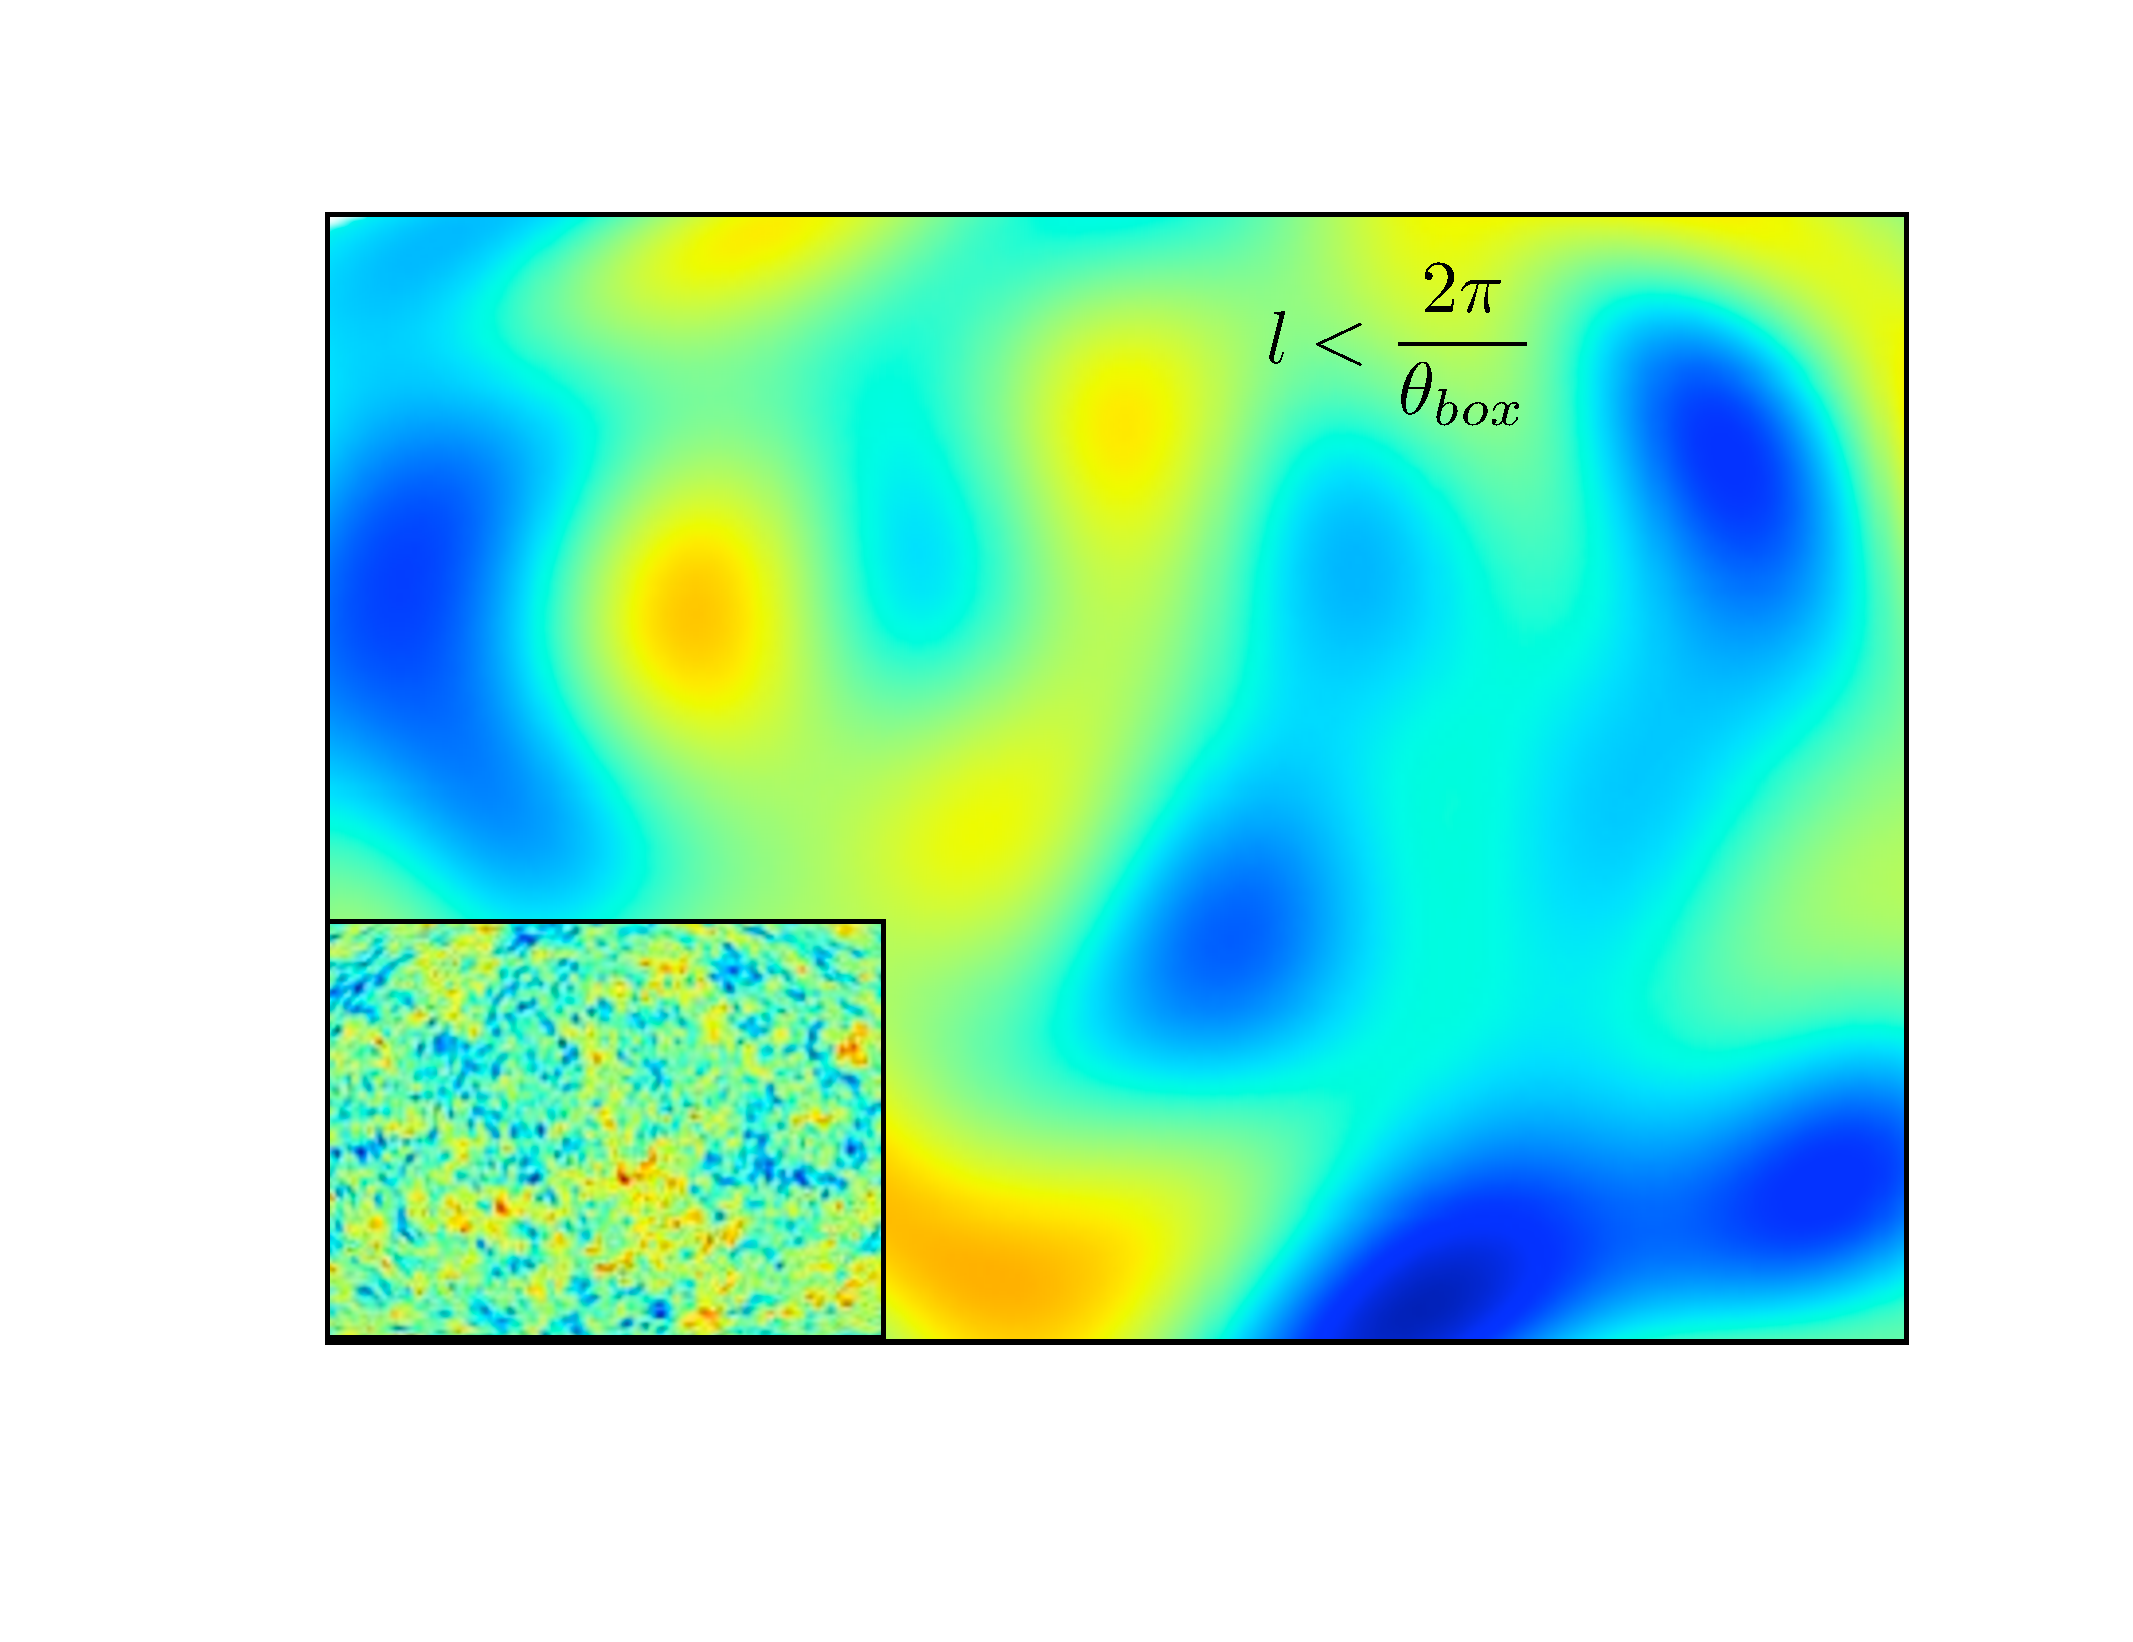
\includegraphics[scale=0.3]{/Users/alessandromanzotti/Work/Astrophysics/Wayne-B_lensing/images/box.pdf}
%\label{default}
\end{center}
\end{figure}


One way to compute the variance is just to sum over all the modes that are super-sample mode considering the width of the box $\theta_{box}\rightarrow l_{max}=\frac{2\pi}{\theta_{box}}$:

\be \label{eqn:lmax}
(\sigma^{\kappa})^{2}=\sum_{0}^{l_{max}=\frac{2\pi}{\theta_{box}}}\frac{2\ell+1}{4\pi}C_{\ell}^{\kappa}
\ee

\begin{figure}[htbp]
\begin{center}
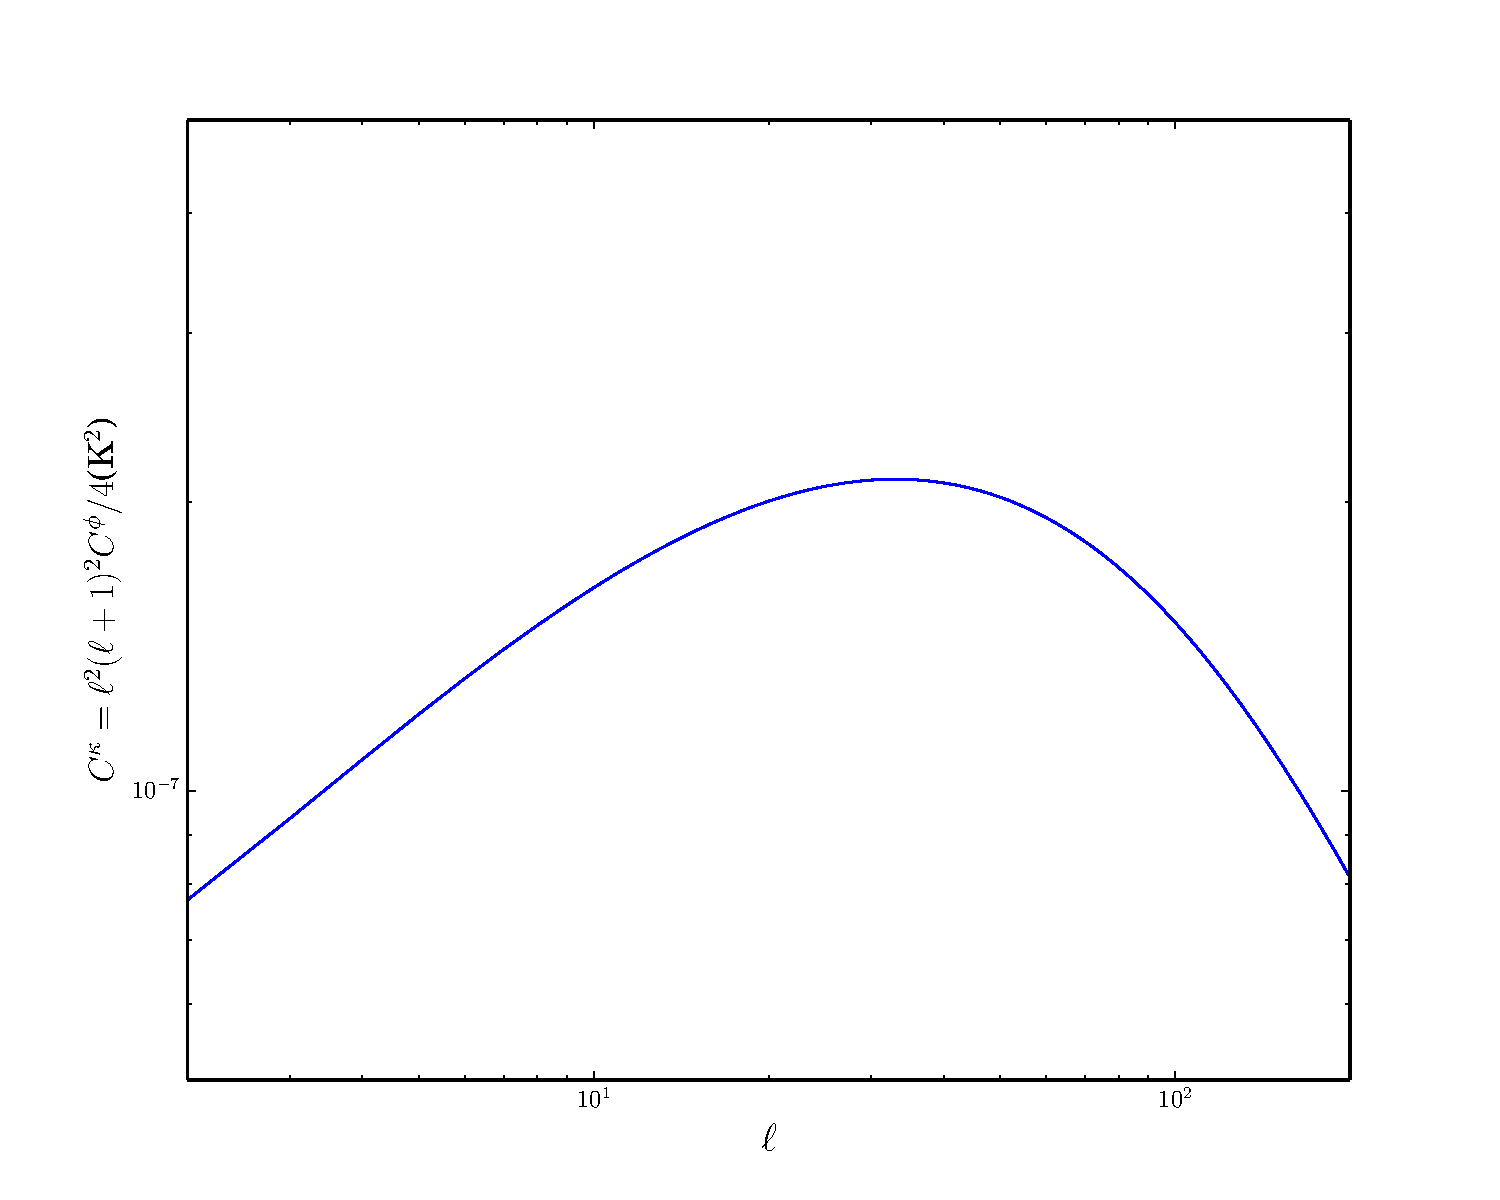
\includegraphics[scale=0.4]{/Users/alessandromanzotti/Work/Astrophysics/Wayne-B_lensing/images/Ckappa.pdf}
\caption{Power spectrum}
%\caption{default}
%\label{default}
\end{center}
\end{figure}

where the convergence power is releted to the lensing one by $C^{\kappa}=\ell^{2}(\ell+1)^{2}C^{\phi}/4$.

Increasing the size of the survey, reduce the number of large scale modes that can be consider as super-survey, and so the variance is reduced. This reduce the ``super sample covariance '' effect. 
Now the width of the survey could be derived from the total area, assuming it covers a circular area, by $\pi \theta_{box}^{2}=\text{Area}(\frac{\pi}{180})^{2}$. 
In this case $l_{max}=\frac{2\pi}{\theta_{box}}=\frac{2\pi}{\sqrt{(\text{tot Area})/\pi} (\pi/180)}=\frac{360\sqrt\pi}{\sqrt{\text{tot Area}}}=\frac{638}{\sqrt{\text{tot Area}}}$, where the total area has to be expressed in degree squared. For a 1000 deg$^{2}$ we get $l_{max}\approx20$

We want to compare this effect to the precision on the measurement of the angular size of sound horizon at last scattering, cause the effect of this background mode can be seen as if the fraction of the sky tested by the survey would have been sitted on a slightly over or under dense region, a slightly closed or open universe. The effect on the power spectrum is the same as a change in the curvature: a shift in the power spectrum.
The current precision reach by planck is $\frac{\sigma_{\theta^{\star}}}{\theta^{\star}}=\frac{0.00006}{1.041}=0.00057$.

We can improve this rough estimate by introducing a simple window function for the survey.

The variance in a 2D flat sky approximation become:
\be
\sigma^{2}_{\kappa}=\int \frac{d^{2}~q}{(2\pi)^{2 }}|\tilde W(q)|^{2} P(q),
\ee
where $\tilde W(q)$ is the fourier transform of the window function (we used the usual Fourier transform conventions).
As a window we can choose a uniform circular disk or radius $R=\theta_{box}$ (normalized so that $\int d^{2}x ~W(x)=1$) in the small angle approximation.
We have
\ba
|\tilde W(q)|&=&\int d^{2}x e^{-i q\cdot x} \Theta(r-R)/(\pi R^{2})\\
&=&\int_{0}^{\infty} x~dx \int_{0}^{2\pi} d\theta e^{-i qx\cos\theta} \Theta(r-R)/(\pi R^{2})\\
&=&1/(\pi R^{2}) \int_{0}^{R} xdx~ \int_{0}^{2\pi} d\theta e^{-i qx\cos\theta} \\
&=&1/(q \pi R^{2}) \int_{0}^{R} xdx~ 2\pi q J_{0}(xq) \\
&=&\frac{2\pi}{\pi R^{2} q^{2}}\int_{0}^{R} d(xq) xq J_{0}(xq) \\
&=&\frac{2\pi}{\pi R^{2} q^{2}}Rq J_{1}(Rq) \\
&=&\frac{2~J_{1}(Rq)}{Rq}. \\
\ea
We have used two properties of bessel functions
\ba
&&J_{n}=\frac{i^{-n}}{\pi}\int_{0}^{\pi}d\theta e^{ix\cos\theta}cos(n\theta)\\
&&\frac{d}{dx}[xJ_{1}(x)]=xJ_{0}(x)\\
\ea


The variance become:
\ba \label{eqn:integral}
\sigma_{\kappa}^{2}&=&\int \frac{d^{2}~\ell}{(2\pi)^{2}} \left(\frac{2~J_{1}(\ell~\theta_{box})}{\ell~\theta_{box}}\right)^{2} C_{\ell}\\
&=&\int \frac{d\ell}{(2\pi)} \ell \left(\frac{2~J_{1}(\ell~\theta_{box})}{\ell~\theta_{box}}\right)^{2} C_{\ell}
\ea
It can also be approximated by a sum 
\be \label{eqn:approx}
\sigma_{\kappa}^{2}=\sum \frac{2\ell+1}{4\pi} \left(\frac{2~J_{1}(\ell~\theta_{box})}{\ell~\theta_{box}}\right)^{2} C_{\ell}.
\ee


\begin{figure}[htbp]
\begin{center}
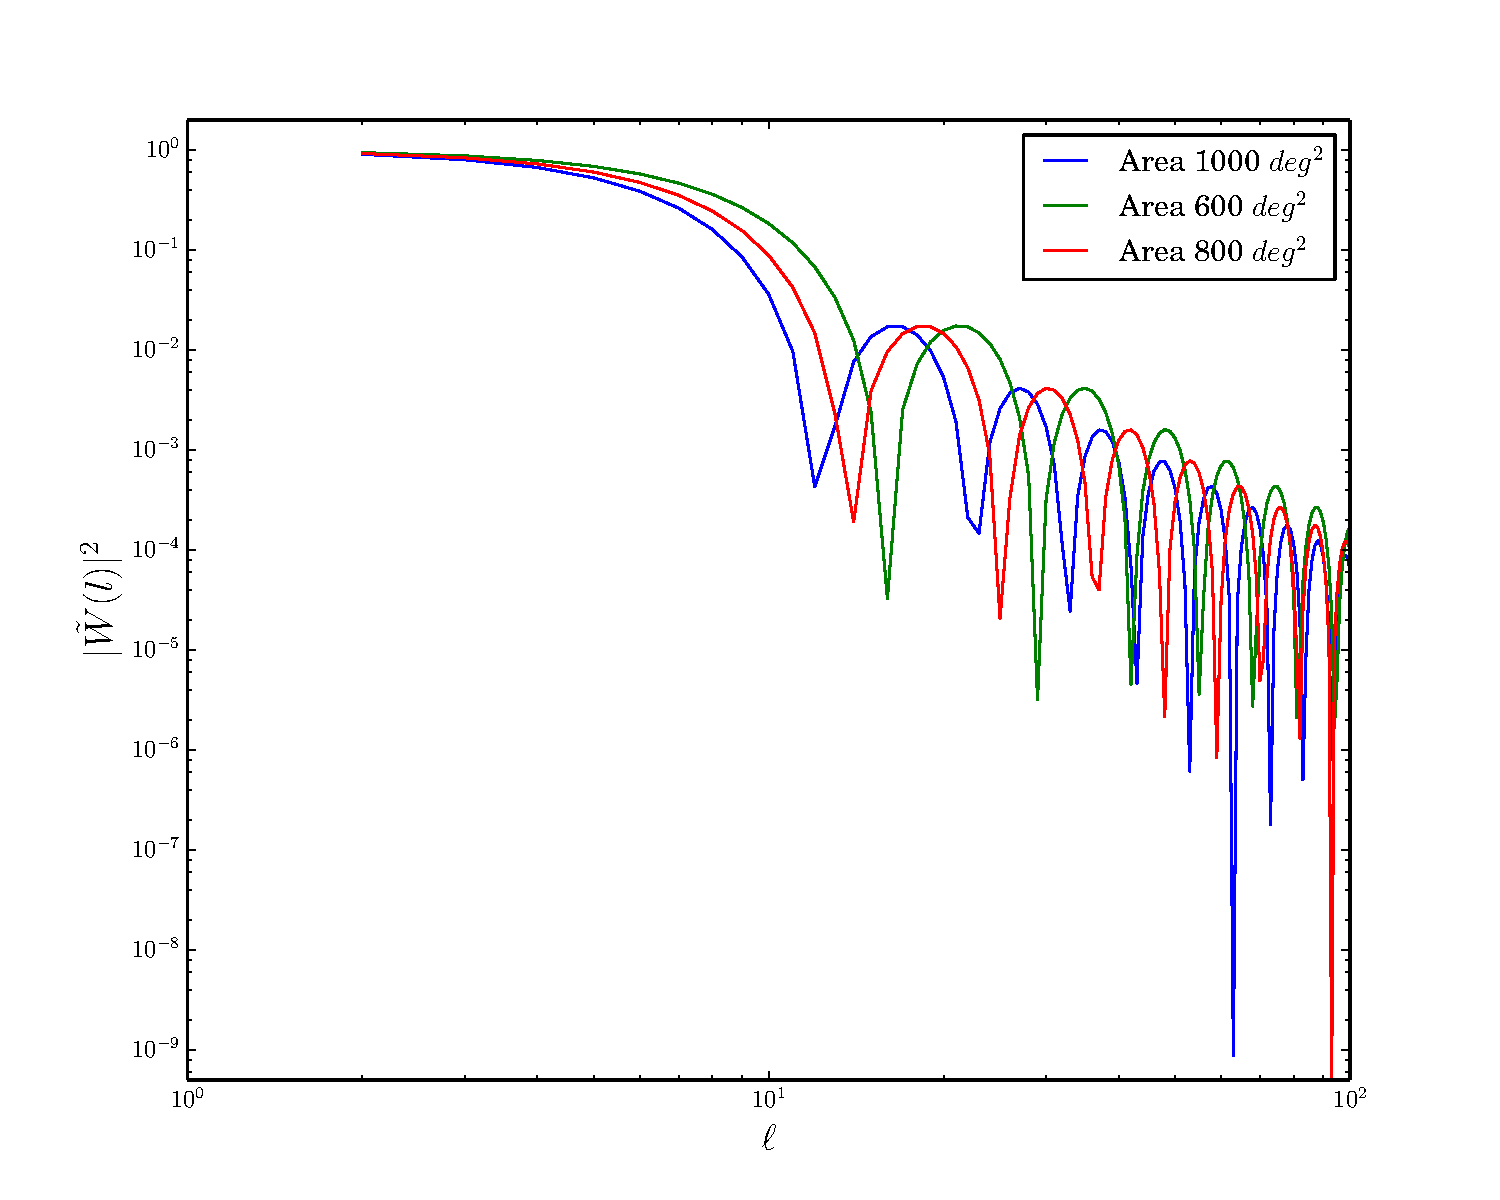
\includegraphics[scale=0.6]{/Users/alessandromanzotti/Work/Astrophysics/Wayne-B_lensing/images/window.pdf}
%\caption{default}
%\label{default}
\end{center}
\end{figure}

\begin{figure}[htbp]
\begin{center}
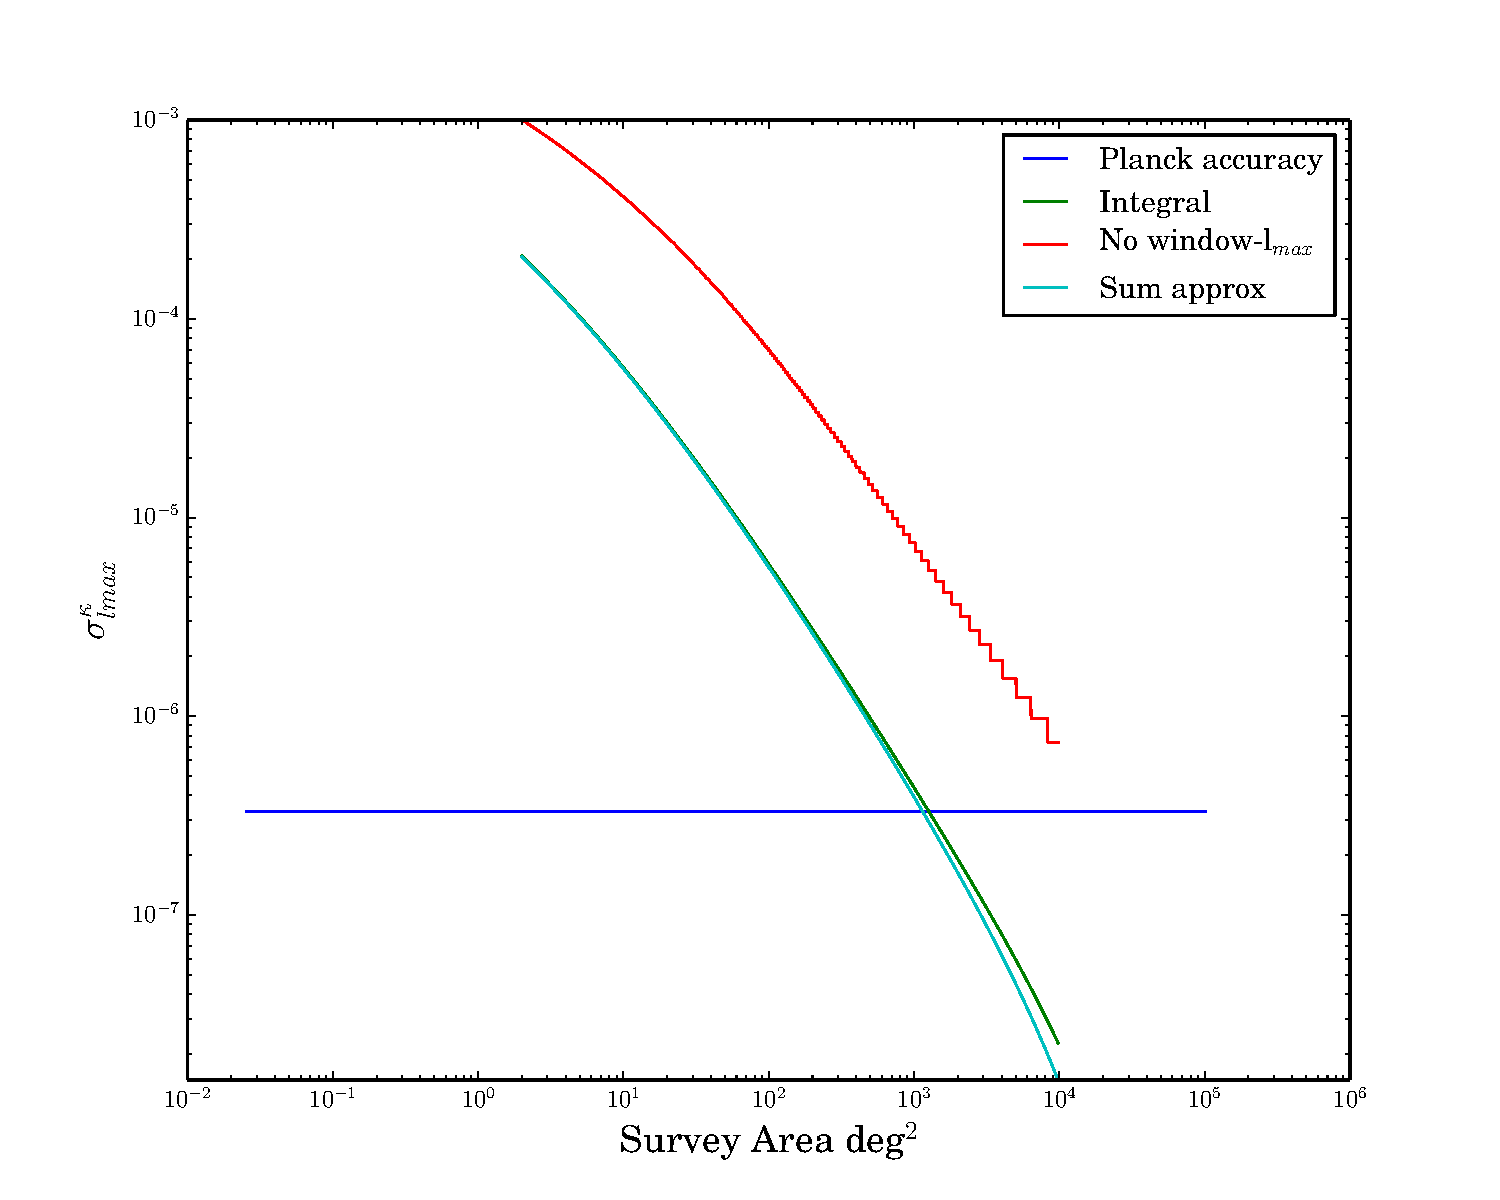
\includegraphics[scale=0.6]{/Users/alessandromanzotti/Work/Astrophysics/Wayne-B_lensing/images/variance.pdf}
\caption{Integral correspond to \refeq{integral} Sum approximation is \refeq{approx} . No window lmax correspond to \refeq{lmax} which I think is pretty different cause it is like having a rectangle window function in Fourier space which give you an un-normalized sync window function in space domain. }
%\label{default}
\end{center}
\end{figure}




\section{Fisher\_estimate}

I compute the value of  $C^{\rm{fid}}_{\ell}$s using CAMB and with those I compute the Fisher estimates of the effect we are looking for, given the accuracy (beam and white noise) of a detector. See Wayne's notes.

The super sample modes shift the CMB power spectrum and so we have:
\begin{equation}
C_l = C_l^{\rm fid} \left[ 1+ \frac{\partial \ln (l^2 C_l^{\rm fid} )}{\partial \ln l} s \right].
\end{equation}
Notice that the effect is stronger where the derivatives are bigger, near the peaks.
Now we can perform a Fisher estimate of $\sigma_s^2$ (no other parameters marignalized) and compare it to $\sigma_\kappa^2$.  
I compute:
\begin{equation}
\frac{\partial C_{\ell}}{\partial s}=C^{\rm fid}\frac{\partial \ln (l^2 C_l^{\rm fid}) }{\partial \ln l},
\end{equation}
directly from the spline function I use to fit the spectrum (maybe we need something more accurate?); after that, following the fisher formalism:
\ben
F_{ss}=\sum_{\ell}\frac{1}{(\delta C_{\ell})^{2}}\left( C^{\rm fid}\frac{\partial \ln (l^2 C_l^{\rm fid} )}{\partial \ln l}\right)^{2}
\een
\ben
F_{ss}=\sum_{\ell}\frac{(2\ell+1)f_{\rm sky}}{2[C^{\rm{fid}}_{\ell}+N_{\ell}]^{2}}\left( C^{\rm fid}\frac{\partial \ln (l^2 C_l^{\rm fid} )}{\partial \ln l}\right)^{2}
\een
assuming SPT-pol 4$\mu K$-arcminute noise and a beam of 1-arcmin:
\be
N_{\ell}=\left( 4 \mu K \left(\frac{\pi}{10800}\right)\right)\exp\{-\ell(\ell+1)\theta\left(\frac{\pi}{10800}\right)/(8\log 2)\}.
\ee
I put the equation explicitly cause I am not sure that when they quote an accuracy they mean this or the same divided by the T$_{CMB}$. Let me know it takes a second to change it (thanks!).

\begin{figure}[htbp]
\begin{center}
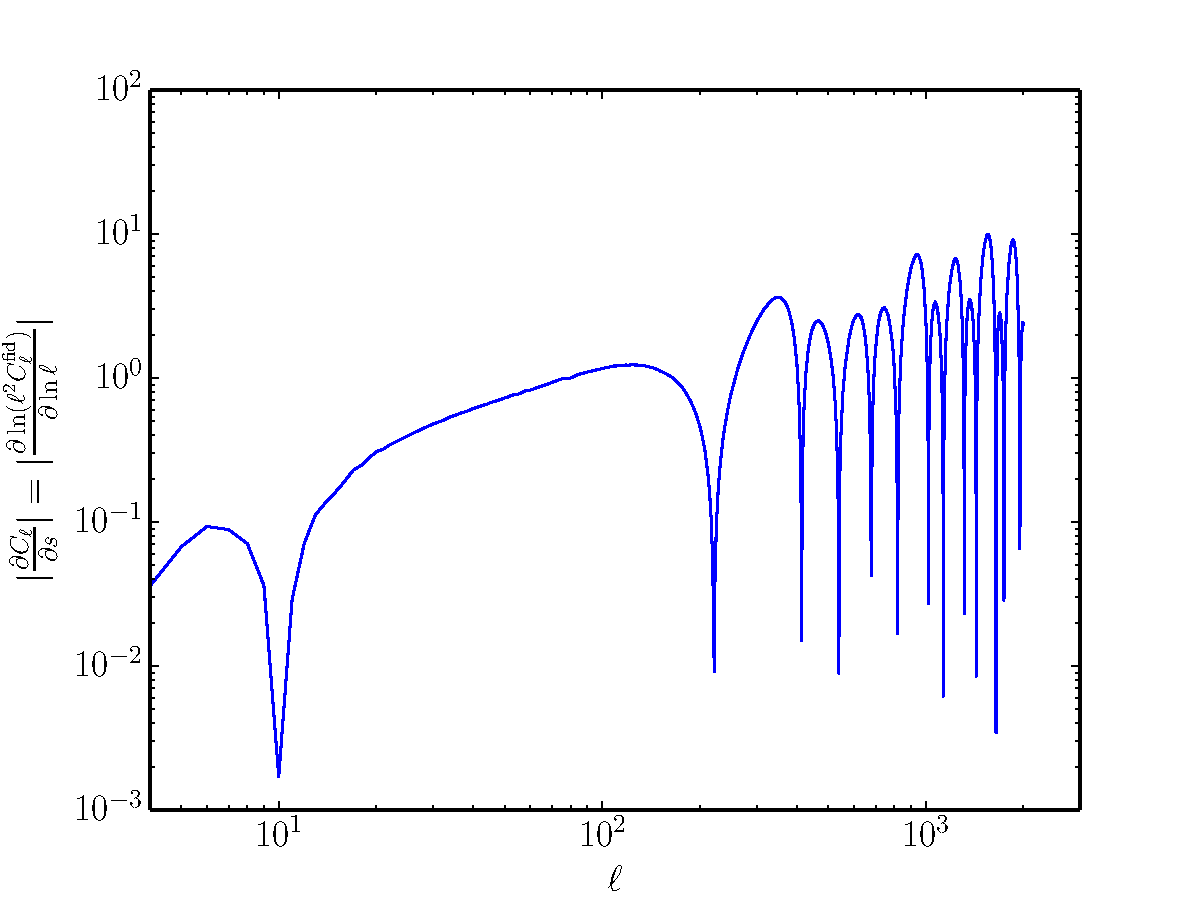
\includegraphics[scale=0.6]{/Users/alessandromanzotti/Work/Astrophysics/Wayne-B_lensing/images/derivatives.pdf}
\caption{Absolute value of the derivatives that enter the fisher matrix computation.}
\label{fig:derivatives}
\end{center}
\end{figure}

\begin{figure}[htbp]
\begin{center}
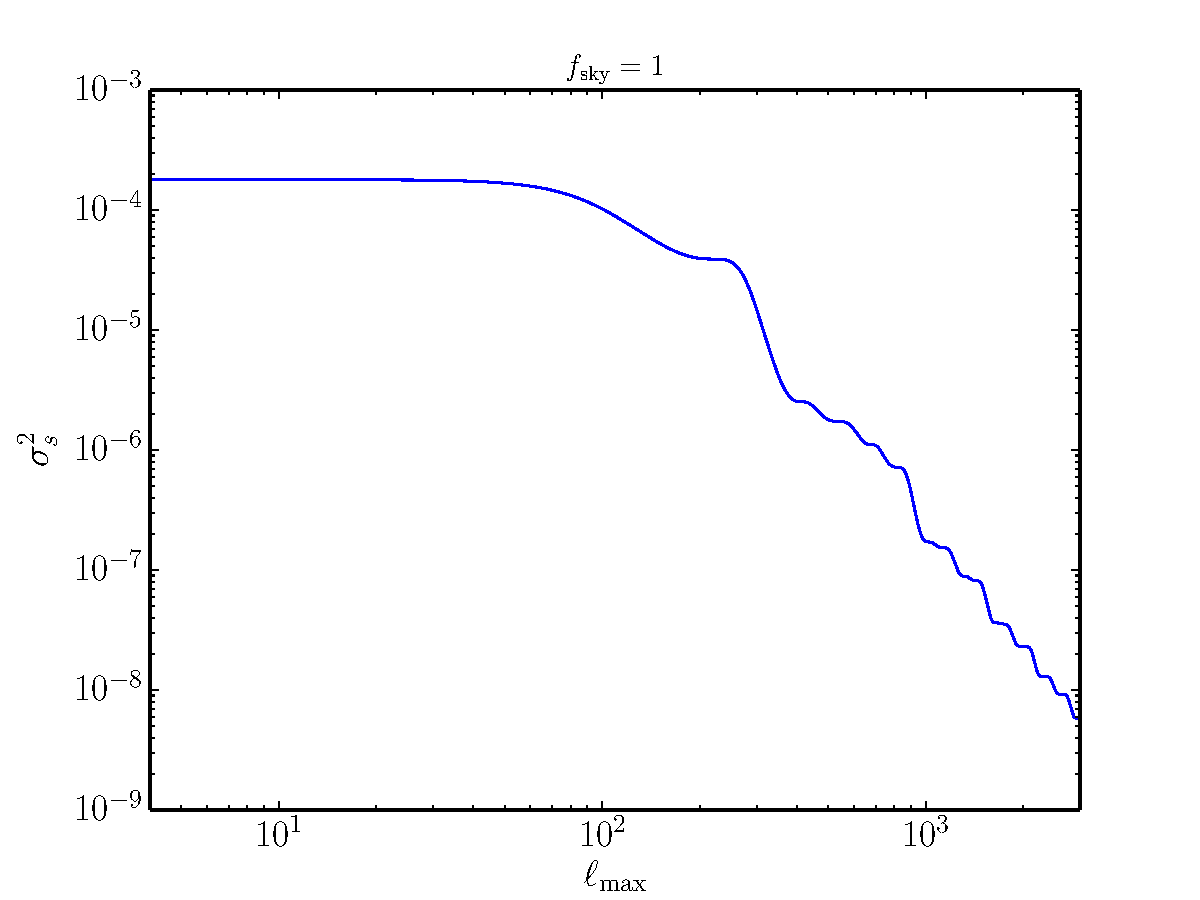
\includegraphics[scale=0.6]{/Users/alessandromanzotti/Work/Astrophysics/Wayne-B_lensing/images/variancefisherfsky.pdf}
\caption{Value of $\sigma^{2}_{s}=\frac{1}{F_{ss}}$ as a function of the maximum multipole considered.}
\label{fig:variancefsky}
\end{center}
\end{figure}

\begin{figure}[htbp]
\begin{center}
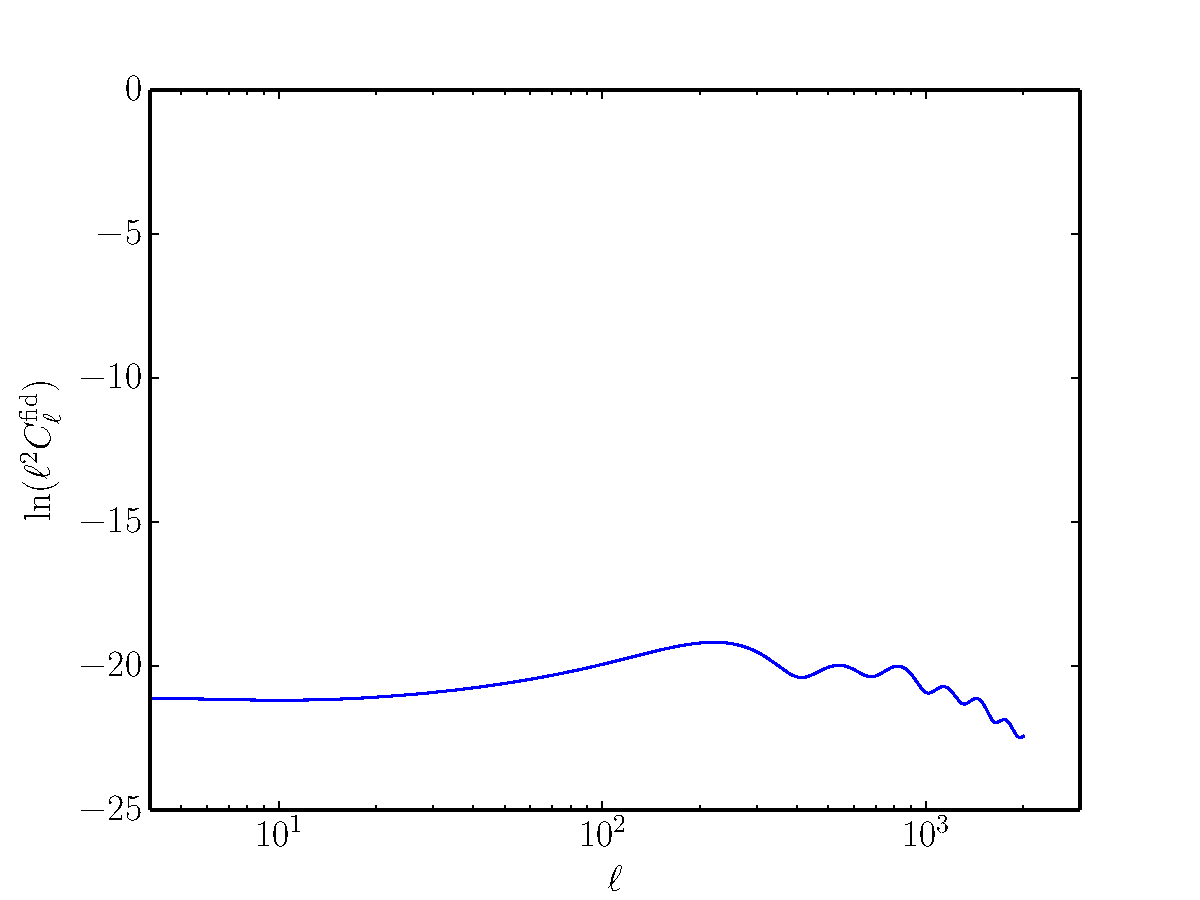
\includegraphics[scale=0.6]{/Users/alessandromanzotti/Work/Astrophysics/Wayne-B_lensing/images/logl2cl.pdf}
%\label{default}
\end{center}
\end{figure}
\begin{figure}[htbp]
\begin{center}
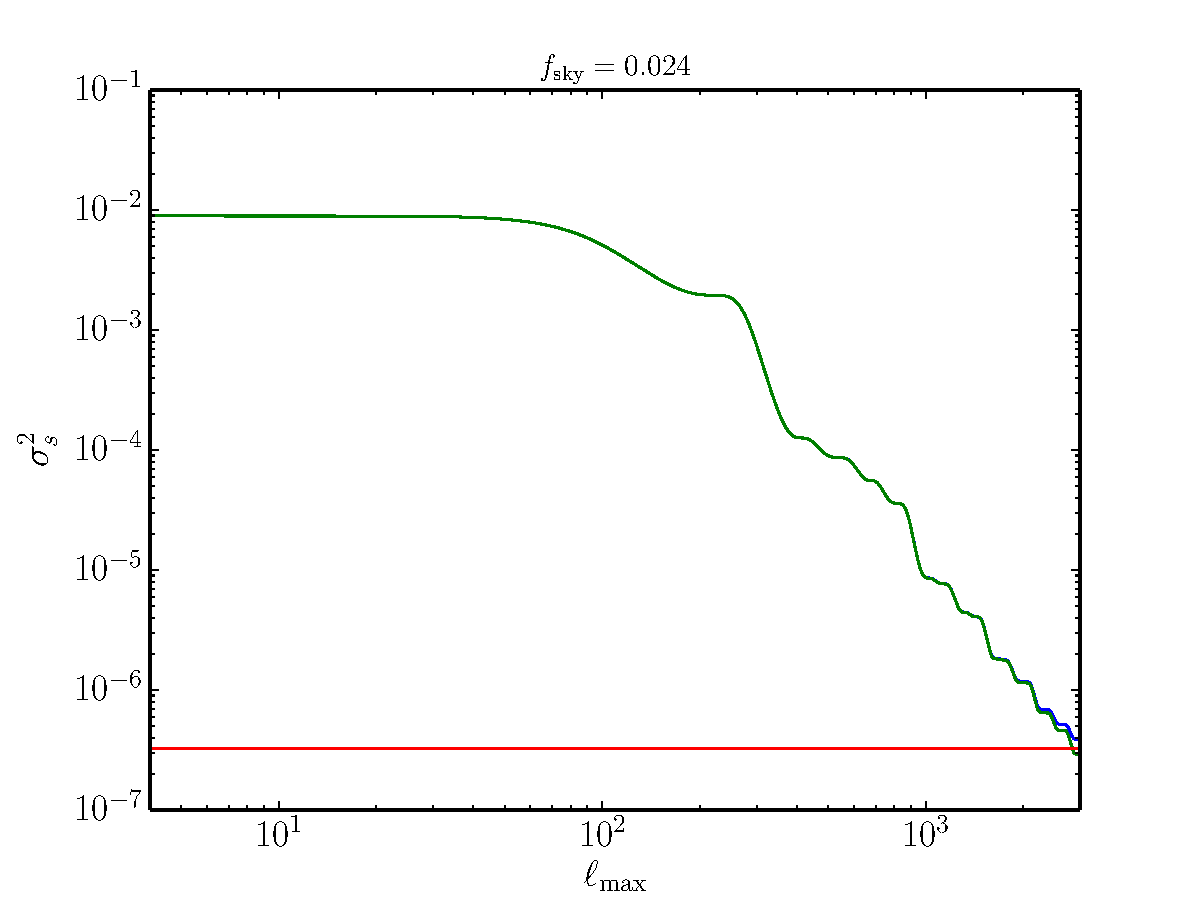
\includegraphics[scale=0.6]{/Users/alessandromanzotti/Work/Astrophysics/Wayne-B_lensing/images/variancefisher.pdf}
\caption{Value of $\sigma^{2}_{s}=\frac{1}{F_{ss}}$ as a function of the maximum multipole considered. $f_{\rm{sky}}$ is chosen considering 1000 deg$^{2}$. Green curve is without instrumental noise, blue take it under consideration. Red line is 
$(\frac{\sigma_{\theta^{\star}}}{\theta^{\star}})^{2}$ for Planck. Note: we are close to the edge, I have to carefully check the noise I used is not wrong or too optimistic.}
%\label{default}
\end{center}
\end{figure}

\end{document}